\documentclass[10pt,twocolumn,twoside]{phdsymp-en}
\usepackage[utf8]{inputenc}
\usepackage[english]{babel}
\usepackage{times}
\usepackage{enumitem}
\usepackage[hang,flushmargin]{footmisc} 
\usepackage{microtype}
\usepackage[dvipsnames]{xcolor}
\usepackage{amsmath}
\usepackage{amssymb}
\usepackage{tikz}
\renewcommand{\baselinestretch}{1.1}
\def\BibTeX{{\rm B\kern-.05em{\sc i\kern-.025em b}\kern-.08em
		T\kern-.1667em\lower.7ex\hbox{E}\kern-.125emX}}
\renewcommand{\familydefault}{\sfdefault}
\usepackage{caption}
\usepackage[list=true]{subcaption}
\usepackage{fontawesome5}
\usepackage[detect-weight=true, binary-units=true, range-phrase=-]{siunitx}
\usepackage{tabularx}
\usepackage{tikz}
\usepackage{tikzscale}
\usepackage[final]{hyperref}
\usepackage{cleveref}

% Table columns.
\newcolumntype{C}{>{\centering\arraybackslash}X}

% Subcaptions.
\captionsetup{compatibility=false}

% Tikz libraries.
\usetikzlibrary{arrows,arrows.meta,automata,calc,shapes.geometric,positioning}

% Terms.
\newcommand{\travisci}{Travis CI}
\newcommand{\velocity}{VeloCIty}

\begin{document}
	\title{Optimising Continuous Integration\\ using Test Case Prioritisation}
	\author{Pieter De Clercq}
	\supervisor{Prof. dr. B. Volckaert, Prof. dr. ir. F. De Turck, J. Vaneessen, D. Kerkhove}
	\maketitle
	
	\begin{abstract}
	Ever since the introduction of traditional software development models in the previous century, the complexity and magnitude of today's software have vastly increased. This evolution has led to the adoption of Agile software development approaches, which pose the need for frequent integration and automated testing. Eventually, this increase in size will also negatively affect the size of the testing suites, resulting in severe scalability issues. This thesis proposes a framework and a novel algorithm for test suite optimisation by prioritising test cases which are likely to fail. The performance has been evaluated on two existing applications, and the results are auspicious.
	\end{abstract}

	\begin{keywords}
		Continuous Integration, test suite, performance, optimisation, prioritisation
	\end{keywords}

	% !TeX root = thesis.tex

\chapter{Introduction}
Given the complexity and rapid pace at which software is being built today, it is inevitable that at some point bugs will emerge. These bugs can either be introduced by a malfunctioning new feature, or by breaking existing functionality (\emph{a regression}). In order to detect bugs in an application before its customers do, an adequate \emph{testing infrastructure} is required.\\

\noindent This testing infrastructure consists of multiple \emph{test cases}, collectively referred to as the \emph{test suite} of the application. The quality of a test suite can be assessed in multiple ways. The first and most used option is to measure which fraction of the source code is tested by at least one test case, a ratio which is expressed as the \emph{coverage} of the application. Another possibility is to apply transformations to the source code and validate whether or not this results in a failed test case, a process indicated as \emph{mutation testing}.\\

\noindent Ideally, this testing process should be automated and performed after every change to the source code. This is generally a very time-consuming occupation, and as such has led to the creation of various automation frameworks and tools, collected under the name of \emph{Continuous Integration} \texttt{[CI]}. Common examples of CI practices are automatically running the test suite and estimating the code coverage after every pushed change to the \emph{Version Control System} \texttt{[VCS]}.\\

\noindent However, applying these practices and maintaining a qualitative test comes at a cost. After every addition or modification to the source code, at least one new test case must be introduced to validate its correctness. As a result of the speed at which the source code tends to grow, the test suite suffers from severe scalability issues. While it is desired and ideally required to execute every single test case in the test suite, there are examples known to literature where this is not possible since this incurs an increasing delay in the development process, which in turn results in economic loss.\\

\noindent Three approaches can be taken towards resolving this issue by reducing the time occupied by waiting for the test results: \tsm{} \texttt{[TSM]}, \tcs{} \texttt{[TCS]} and \tcp{} \texttt{[TCP]}. The main subject of this thesis will be to implement a framework for TCP. To accomplish this, the next chapter will introduce important concepts which are used in modern software engineering. \autoref{chap:related-work} will elaborate on the aforementioned approaches and present accompanying algorithms. The implementation details of the new framework will be discussed in \autoref{chap:velocity}. Afterwards, \autoref{chap:evaluation} will evaluate the performance of this framework and provide insights to the characteristics of a typical test suite. More specifically, this chapter will research the probability of (repeated) test failure and the average duration of a test run. Finally, \autoref{chap:conclusion} will present additional ideas and improvements to the framework.
	\section{Technieken}
\noindent Deze masterproef presenteert drie technieken om dit schaalbaarheidsprobleem op te lossen.

\begin{figure*}[t]
	\centering
	\subcaptionbox{Testpakket Minimalisering}{\includegraphics[width=0.32\textwidth]{assets/tsm.tikz}}
	\hfill
	\subcaptionbox{Test Selectie}{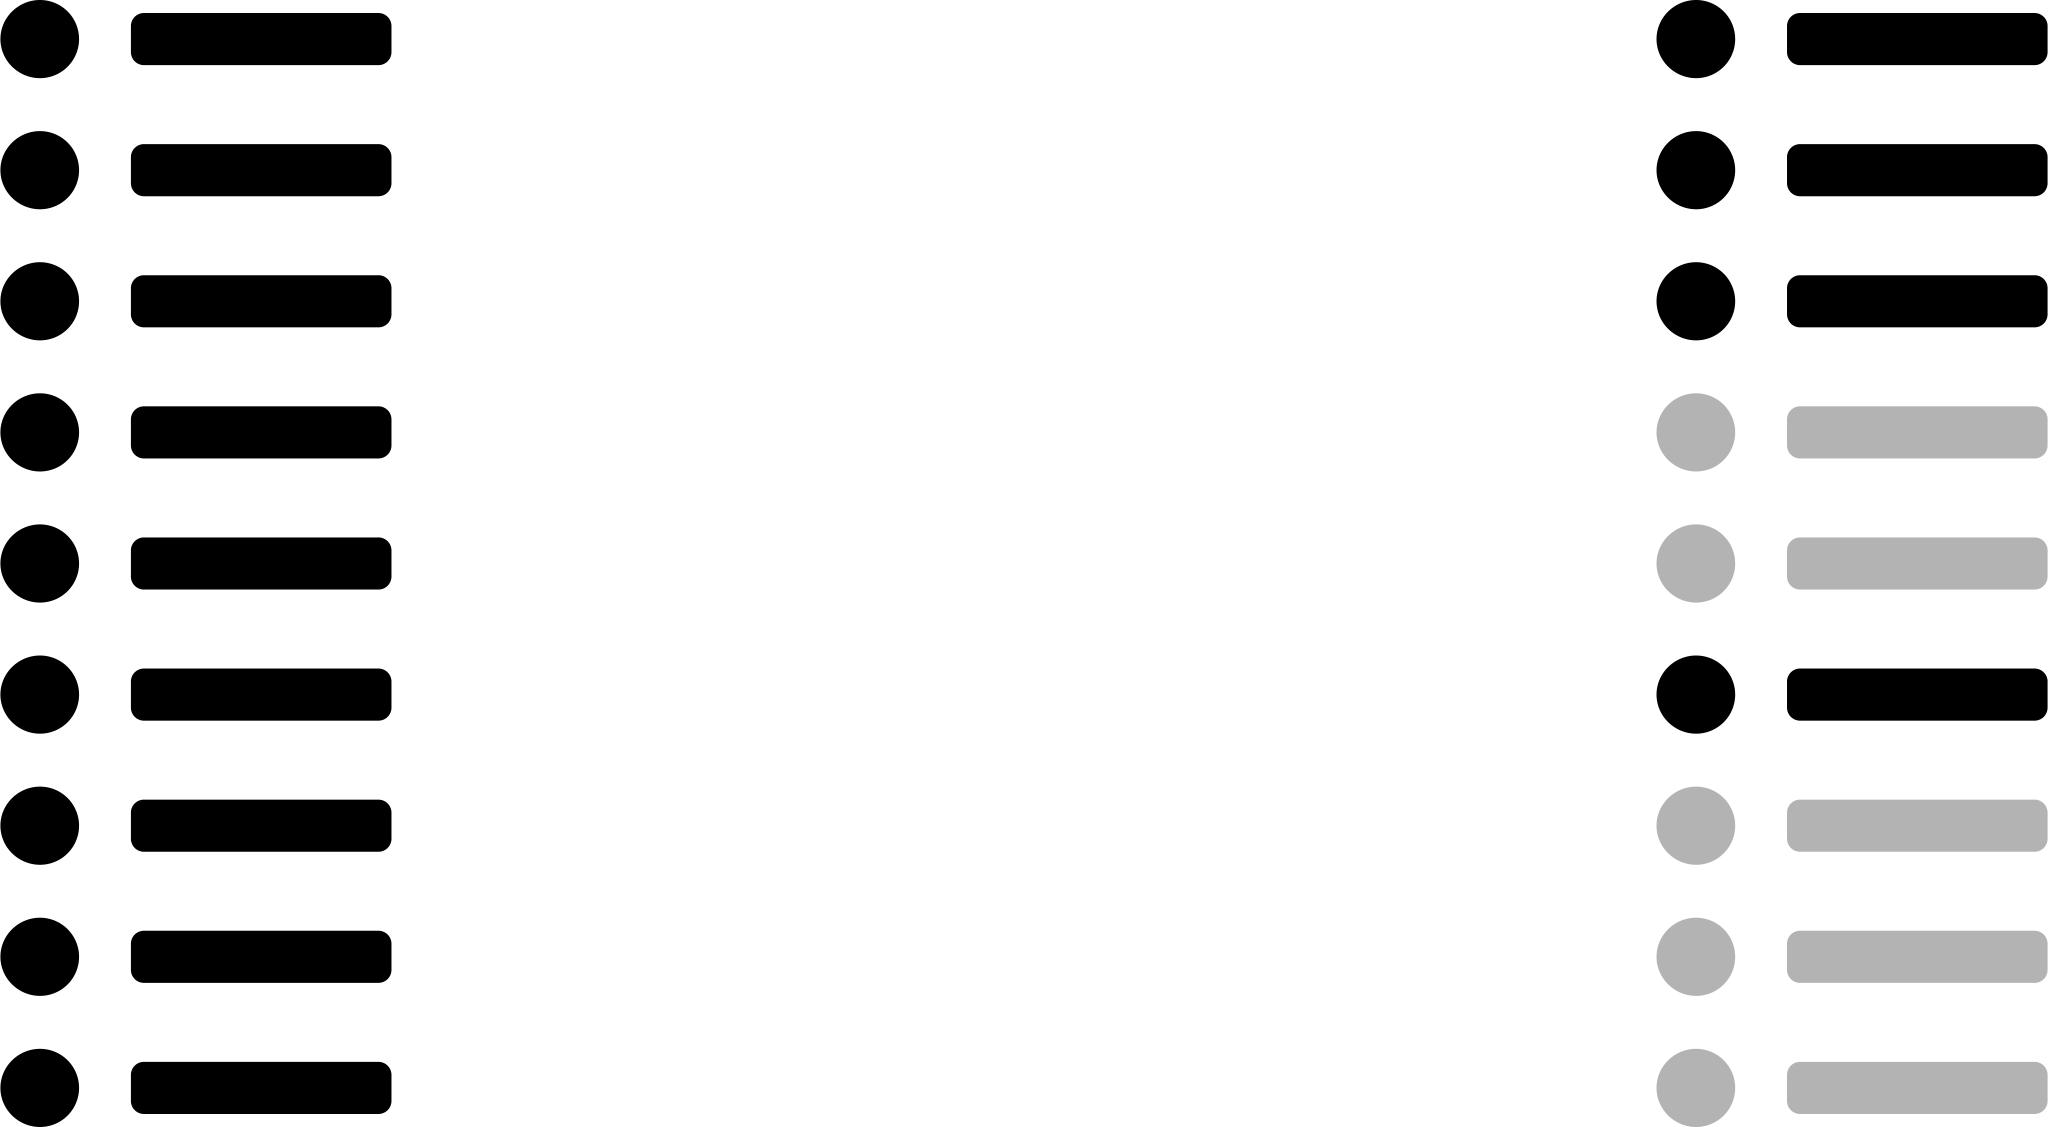
\includegraphics[width=0.32\textwidth]{assets/tcs.tikz}}
	\hfill
	\subcaptionbox{Test Prioritering}{\includegraphics[width=0.32\textwidth]{assets/tcp.tikz}}
	\caption{Overzicht van de technieken.}
\end{figure*}

\subsection{Testpakket Minimalisering (TSM)}
\noindent De eerste techniek is Testpakket Minimalisering (TSM) \cite{10.1002/stv.430}. TSM probeert de grootte van het testpakket te verkleinen door redundante tests permanent te verwijderen, volgens volgende definitie:\\

\noindent\fbox{\begin{minipage}{\dimexpr\columnwidth-2\fboxsep-2\fboxrule\relax}
\textbf{Gegeven:}
\begin{itemize}[leftmargin=1em]
	\item $T = \{t_1, \dots, t_n\}$ een testpakket bestaande uit tests $t_j$.
	\item $R = \{r_1, \dots, r_m\}$ een verzameling vereisten die voldaan moeten zijn om te stellen dat een applicatie grondig getest is.
	\item $\{T_1, \dots, T_m\}$ deelverzamelingen van tests uit $T$. Voor $i \in [1..m]$ wordt elke deelverzameling $T_i$ wordt geassocieerd met een vereiste $r_i$, zodanig dat eender welke test $t_j \in T_i$ kan worden uitgevoerd om te voldoen aan vereiste $r_i$.
\end{itemize}
\mbox{}\\
Het probleem van TSM is vervolgens gedefinieerd als het vinden van een minimale deelverzameling $T'$ van tests $t_j \in T$, zodanig dat aan elke vereiste $r_i \in R$ voldaan is.
\end{minipage}}

\subsection{Test Selectie (TCS)}
\noindent In plaats van tests permanent te verwijderen, is het ook mogelijk om de veranderingen aan de code te analyseren om zo te bepalen welke tests zeker uitgevoerd moeten worden. Analoog kunnen andere tests mogelijk worden uitgesloten, omdat ze (waarschijnlijk) niet zullen falen \cite{10.1002/stv.430}.\\

\noindent\fbox{\begin{minipage}{\dimexpr\columnwidth-2\fboxsep-2\fboxrule\relax}
\textbf{Gegeven:}
\begin{itemize}[leftmargin=1em]
	\item $T$ het testpakket.
	\item $P$ de vorige versie van de code.
	\item $P'$ the huidige (aangepaste) versie van de code.
\end{itemize}
\mbox{}\\
TCS vindt een deelverzameling $T' \subseteq T$ die gebruikt kan worden om $P'$ adequaat te testen. 
\end{minipage}}

\subsection{Test Prioritering (TCP)}
\noindent TSM en TCS voeren zo weinig mogelijk tests uit om de omvang van het testpakket te verkleinen. Soms kan het echter gewenst zijn om toch elke test uit te voeren, bijvoorbeeld bij kritische software voor medische doeleinden. In dit geval kan het testpakket nog steeds geoptimaliseerd worden, door de uitvoeringsvolgorde aan te passen. Test Prioritering (TCP) \cite{10.1002/stv.430} rangschikt de tests zodanig dat een vooropgesteld doel zo snel mogelijk bereikt wordt. In deze masterproef zal het doel steeds zijn om zo snel mogelijk een falende test te detecteren.\\

\noindent\fbox{\begin{minipage}{\dimexpr\columnwidth-2\fboxsep-2\fboxrule\relax}
\textbf{Gegeven:}
\begin{itemize}[leftmargin=1em]
	\item $T$ het testpakket.
	\item $PT$ de verzameling van alle permutaties van $T$.
	\item $f: PT \mapsto \mathbb{R}$ een functie die gebruikt wordt om permutaties met elkaar te vergelijken.
\end{itemize}
\mbox{}\\
TCP bepaalt de optimale permutatie $T' \in PT$ zodanig dat $\forall T'' \in PT : f(T') \ge f(T'') \Rightarrow (T'' \ne T')$. 
\end{minipage}}
	% !TeX root = ../thesis.tex

\section{Algorithms}
In \autoref{ssec:tsm} the relation was explained between applying Test Suite Minimisation and finding the minimal hitting set of the test suite and the set of requirements, which is an NP-complete problem. Therefore, the use of \emph{heuristics} is required. A heuristic is an experience-based method that can be used to solve a hard to compute problem by finding a fast approximation \cite{6588537}. However, the found solution will mostly be suboptimal or might sometimes even fail to find any solution at all. Considering its relation to the minimal hitting set problem, heuristics that are known to literature for solving this problem can also be used to implement \tsm{}. A selection of these heuristics will be discussed below. It should be noted however that the used terminology and naming of the variables might have been changed to ensure mutual consistency. Every algorithm has been modified to adhere to the conventions provided in \autoref{def:alg-naming} and \autoref{def:cardinality}.

\begin{definition}[Naming convention]
\label{def:alg-naming}
\mbox{}
\begin{itemize}
	\item $C$: the set of all lines in the application source code that are covered by at least one test case $t \in TS$.
		\begin{itemize}
			\item $CT_l$ denotes the test group $l$, which corresponds to the set of all tests $t \in TS$ that cover source code line $l \in C$.
		\end{itemize}
	\item $RS$: the representative set of test cases, these are the test cases that have been selected by the algorithm.
	\item $TS$: the set of all test cases in the test suite.
		\begin{itemize}
			\item $TL_t$ denotes the set of all source code lines that are covered by test $t \in TS$.
		\end{itemize}
\end{itemize}
\end{definition}

\begin{definition}[Cardinality]
\label{def:cardinality}
For a finite set $S$, the cardinality $|S|$ is defined as the number of elements in $S$. In case of potential confusion, the cardinality of $S$ can also be denoted as $Card(S)$.
\end{definition}

% !TeX root = ../../thesis.tex

\subsection{Greedy algorithm}
\label{ssec:alg-greedy}
The first algorithm is a \emph{greedy} heuristic, which was originally designed by Chvatal to find an approximation for the set-covering problem \cite{evaluationoftestsuiteminimization}. A greedy algorithm always makes a locally optimal choice, assuming that this will eventually lead to a globally optimal solution \cite{10.5555/1614191}. Algorithm \ref{alg:tsm-greedy} presents the Greedy algorithm for \tsm{}. The goal of the algorithm is to construct a set of test cases that cover every line in the code, by requiring as few tests as possible.\\

\noindent Initially, the algorithm starts with an empty result set $RS$, the set $TS$ of all test cases and the set $C$ of all coverable source code lines. Furthermore, $TL_t$ denotes the set of source code lines in $C$ that are covered by test case $t \in TS$. Subsequently, the algorithm iteratively selects test cases from $TS$ and adds them to $RS$. The locally optimal choice is to always select the test case that will contribute the most still uncovered lines, ergo the test $t$ for which the cardinality of the intersection between $C$ and $TL_t$ is maximal. After every iteration, the now covered lines $TL_t$ are removed from $C$ and the selection process is repeated until $C$ is empty. Upon running the tests, only the tests in $RS$ must be executed. This algorithm can be converted to make it applicable to \tcp{} by converting the set $RS$ to a list to maintain the order in which the test cases were selected, which is equivalent to the prioritised order of execution.

\begin{algorithm}[h!]
\caption{Greedy algorithm for \tsm{}}
\label{alg:tsm-greedy}
\begin{algorithmic}[1]
	\State {\bfseries Input:} Set $TS$ of all test cases, set $C$ of all source code lines that are covered by any $t \in TS$ and $TL_t$ the set of all lines are covered by test case $t \in TS$.
	\State {\bfseries Output:} Subset $RS \subseteq TS$ of tests to execute.
	\State $RS \gets \emptyset$
	\While{$C \neq \emptyset$}
		\State $t\_max \gets 0$
		\State $tl\_max \gets \emptyset$
		
		\ForAll{$t \in TS$}
			\State $tl\_current \gets C \cap TL_{t}$
			\If{$|tl\_current| > |tl\_max|$}
				\State $t\_max \gets t$
				\State $tl\_max \gets tl\_current$
			\EndIf
		\EndFor
		
		\State $RS \gets RS \cup \{t\_max\}$
		\State $C \gets C \setminus tl\_max$
	\EndWhile
\end{algorithmic}
\end{algorithm}

% !TeX root = ../../thesis.tex

\subsection{HGS}\label{ssec:alg-hgs}
The second algorithm was created by Harrold, Gupta and Soffa \cite{hgs}. This algorithm constructs the minimal hitting set of the test suite in an iterative fashion. As opposed to the greedy algorithm (\autoref{ssec:alg-greedy}), the HGS algorithm considers the test groups $CT$ instead of the set $TLt$ to obtain a list of test cases that cover all source code lines. More specifically, this algorithm considers the distinct test groups, denoted as $CTD$. Two test groups are considered indistinct if they differ in at least one test case. The pseudocode for this algorithm is provided in Algorithm \autoref{alg:hgs}.\\

\noindent Similar to the previous algorithm, an empty representative set $RS$ is constructed in which the selected test cases will be stored. The algorithm begins by iterating over every source code line $l \in C$ and constructing the corresponding set of test groups $CT_l$. As mentioned before, for performance reasons this set is reduced to $CTD$, only retaining distinct test groups. Next, the algorithm selects every test group of which the cardinality is equal to 1 and adds these to $RS$. This corresponds to every test case that covers a line of code, which is exclusively covered by that single test case. Subsequently, the lines that are covered by any of the selected test cases are removed from $C$. This process is repeated for an incremented cardinality, until every line in $C$ is covered. Since the remaining test groups will now contain more than one test case, the algorithm needs to make a choice on which test case to select. The authors have chosen that the test case that occurs in the most test groups is preferred. In the event of a tie, this choice is deferred until the next iteration.\\

\noindent The authors have provided an accompanying calculation of the computational time complexity of this algorithm \cite{hgs}. With respect to the naming convention introduced in \autoref{def:alg-naming}, additionally let $n$ denote the number of distinct test groups $CTD$, $nt$ the number of test cases $t \in TS$ and $MAX\_CARD$ the cardinality of the largest test group. The HGS algorithm consists of two steps which are performed repeatedly. The first step involves computing the number of occurrences of every test case $t$ in each test group. Given that there are $n$ distinct test groups and, in the worst case scenario, each test group can contain $MAX\_CARD$ test cases which all need to be examined once, the computational cost of this step is equal to $O(n * MAX\_CARD)$. In order to determine which test case should be included in the representative set $RS$, the algorithm needs to find all test cases for which the number of occurrences in all test groups is maximal, which requires at most $O(nt * MAX\_CARD)$. Since every repetition of these two steps adds a test case that belongs to at least one out of $n$ test groups to the representative set, the overall runtime of the algorithm is $O(n * (n + nt) * MAX\_CARD)$.
\begin{algorithm}[h!]
\caption{HGS algorithm (\cite{hgs})}
\label{alg:hgs}
\begin{algorithmic}[1]
	\State {\bfseries Input:} Distinct test groups $T_1, \dots T_n \in CDT$, containing test cases from $TS$.
	\State {\bfseries Output:} Subset $RS \subseteq TS$ of tests to execute.
	\State $marked \gets array[1 \dots n]$ \Comment{initially $false$}
	\State $MAX\_CARD \gets max \{Card(T_i) \vert T_i \in CDT\}$
	\State $RS \gets \bigcup \{ T_i \vert Card(T_i) = 1 \}$
	\ForAll{$T_i \in CDT$}
		\If{$T_i \cap RS \neq \emptyset$} $marked[i] \gets true$ \EndIf
	\EndFor
	\State $current \gets 1$
	\While{$current < MAX\_CARD$}
		\State $current \gets current + 1$
		\While{$\exists T_i : Card(T_i) = current, marked[i] = false$}
			\State $list \gets \{t \vert t \in T_i : Card(T_i) = current, marked[i] = false\}$
			\State $next \gets SelectTest(current, list)$
			\State $reduce \gets false$
			\ForAll{$T_i \in CDT$}
				\If{$next \in T_i$}
					\State $marked[i] = true$
					\If{$Card(T_1) = MAX\_CARD$} $reduce \gets true$ \EndIf
				\EndIf
			\EndFor
			\If{$reduce$}
				\State $MAX\_CARD \gets max \{Card(T_i) \vert marked[i] = false\}$
			\EndIf
			\State $RS \gets RS \cup \{next\}$
		\EndWhile
	\EndWhile
	
	\Function{SelectTest}{$size$, $list$}
		\State $count\gets array[1 \dots nt]$
		
		\ForAll{$t \in list$}
			\State $count[t] \gets |\{T_j \vert t \in T_j, marked[T_j] = false, Card(T_j) = size\}|$
		\EndFor
		
		\State $tests \gets \{t \vert t \in list, count[t] = max(count) \}$
		
		\If{$|tests| = 1$} \Return $tests[0]$
		\ElsIf{$|tests| = MAX\_CARD$} \Return $tests[0]$
		\Else{} \Return $SelectTest(size+1, tests)$
		\EndIf
	\EndFunction
\end{algorithmic}
\end{algorithm}
% !TeX root = ../../thesis.tex

\subsection{ROCKET algorithm}
\label{ssec:alg-rocket}

The third and final algorithm is the ROCKET algorithm. This algorithm has been presented by Marijan, Gotlieb and Sen \cite{6676952} as part of a case study to improve the testing efficiency of industrial video conferencing software. Contrarily to the previous algorithms, which attempted to execute as few test cases as possible, this algorithm does execute the entire test suite. Unlike the previous algorithms that only take code coverage into account, this algorithm also considers historical failure data and test execution time. The objective of this algorithm is twofold: select the test cases with the highest successive failure rate, while also maximising the number of executed test cases in a limited time frame. In the implementation below, we will consider an infinite time frame as this is a domain-specific constraint and irrelevant for this thesis. This algorithm will yield a total ordering of all the test cases in the test suite, ordered using a weighted function.\\

\noindent The modified version of the algorithm (of which the pseudocode is provided in \Cref{alg:rocket}) takes three inputs:
\begin{itemize}
	\item $TS = \{T_1, \dots, T_n\}$: the set of test cases to prioritise.
	\item $E = \begin{bmatrix}
		E_1 & \dots & E_n
	\end{bmatrix}$: the execution time of each test case.
	\item $F = \begin{bmatrix}
		F_1 & \dots & F_n
	\end{bmatrix}$: the failure statuses of each test case.
		\begin{itemize}
			\item $F_t = \begin{bmatrix}
				f_1 & \dots & f_m
			\end{bmatrix}$: the failure status of test case $t$ over the previous $m$ successive executions. $F_{ij} = 1$ if test case $i$ has failed in execution $(current - j)$, $0$ if it has passed.
		\end{itemize}
\end{itemize}

\noindent The algorithm starts by creating an array $P$ of length $n$, which contains the priority of each test case. The priority of each test case is initialised at zero. Next, we construct an $m \times n$ failure matrix $MF$ and fill it using the following formula.
\[
	MF[i, j] = \left\{
	\begin{array}{rl}
		1 & \text{if } F_{ji} = 1 \\
		-1 & \text{otherwise} \\
		\end{array}
	\right.
\]

\noindent \Cref{tbl:rocket-failurematrix} contains an example of this matrix $MF$. In this table, we consider the hypothetical failure rates of the last two executions of six test cases.

\begin{table}[h]
\centering
\begin{tabular}{| l || c | c | c | c | c | c |}
	\hline
	\textbf{run} & \textbf{$T_1$} & \textbf{$T_2$} & \textbf{$T_3$} & \textbf{$T_4$} & \textbf{$T_5$} & \textbf{$T_6$}\\\hline
	$current - 1$ & $1$ & $1$ & $1$ & $1$ & $-1$ & $-1$\\
	$current - 2$ & $-1$ & $1$ & $-1$ & $-1$ & $1$ & $-1$\\
	\hline
\end{tabular}
\caption{Example of the failure matrix $MF$.}
\label{tbl:rocket-failurematrix}
\end{table}

\noindent Afterwards, we fill $P$ with the cumulative priority of each test case. We can calculate the priority of a test case by multiplying its failure rate with a domain-specific weight heuristic $\omega$. This heuristic reflects the probability of repeated failures of a test case, given earlier failures. In their paper \cite{6676952}, the authors apply the following weights:

\[
	\omega_i = \left.
	\begin{cases}
		0.7 & \text{if } i = 1 \\
		0.2 & \text{if } i = 2 \\
		0.1 & \text{if } i >= 3 \\
	\end{cases}
	\right.
\]
$$P_j = \sum_{i = 1 \dots m} MF[i, j] * \omega_i$$

\noindent Finally, the algorithm groups test cases based on their calculated priority in $P$. Every test case that belongs to the same group is equally relevant for execution in the current test run. However, within every test group, the test cases will differ in execution time $E$. The final step is to reorder test cases that belong to the same group in such a way that test cases with a shorter duration are executed earlier in the group.

\begin{algorithm}[h!]
\caption{ROCKET algorithm}
\label{alg:rocket}
\begin{algorithmic}[1]
	\State {\bfseries Input:} Set $TS = \{T_1, \dots, T_n\}$ of all test cases,

	Execution time $E_t$ of every test case,
	
	Failure status $F$ for each test case over the previous $m$ successive iterations.
	\State {\bfseries Output:} Priority of test cases $P$.
	\State $P \gets array[1 \dots n]$ \Comment{initially $0$}
	\State $MF \gets array[1 \dots m]$
	\ForAll{$i \in 1 \dots m$}
		\State $MF[i] \gets array[1 \dots n]$
		\ForAll{$j \in 1 \dots n$}
			\If{$F[j][i] = 1$}
				$MF[i][j] \gets -1$
			\Else{}
				$MF[i][j] \gets 1$
			\EndIf
		\EndFor
	\EndFor
	\ForAll{$j \in 1 \dots n$}
		\ForAll{$i \in 1 \dots m$}
			\If{$i = 1$}
				$P[j] \gets P[j] + (MF[i][j] * 0.7)$
			\ElsIf{$i = 2$}
				$P[j] \gets P[j] + (MF[i][j] * 0.2)$
			\Else{}
				$P[j] + (MF[i][j] * 0.1)$
			\EndIf
		\EndFor
	\EndFor
	\State $Q \gets \{P[j] \vert j \in 1 \dots n\}$ \Comment{distinct priorities}
	\State $G \gets array[1 \dots Card(Q)]$ \Comment{initially empty sets}
	\ForAll{$j \in 1 \dots n$}
		\State $p \gets P[j]$
		\State $G[p] \gets G[p] \cup \{j\}$
	\EndFor
	\State Sort every group in $G$ based on ascending execution time in $E$.
	\State Sort $P$ according to which group it belongs and its position within that group.
\end{algorithmic}
\end{algorithm}

	\section{Framework}
\noindent This thesis proposes \velocity{} as a language-agnostic framework that enables Test Case Prioritisation on existing software projects. The architecture consists of three main components, a meta predictor, and a novel prioritisation algorithm.

\subsection{Agent}
\noindent The first component is the agent. This component hooks into the testing framework of the application to execute the test cases in the required order. The agent obtains the optimal execution sequence by communicating with the next component, which is the controller.

\subsection{Controller}
\noindent The controller is a daemon which performs two tasks. First, the controller listens for requests from agents and acts as a relay to the predictor daemon. Additionally, the controller receives feedback from the agent after every executed test run. This information is used to update the meta predictor, which will be described later.

\subsection{Predictor}
\noindent The final main component of the architecture is the predictor daemon. This component is responsible for interpreting the code changes and determining the optimal order of execution using ten built-in prediction algorithms. These algorithms are variations of the three discussed algorithms, as well as the Alpha algorithm.

\subsection{Meta predictor}
\noindent Since the predictor daemon contains multiple prediction algorithms, a small extra component is required to decide which sequence should be preferred as the final execution order. The meta predictor is a table which assigns a score to every prediction algorithm. The final execution order is the one that has been predicted by the prediction algorithm with the highest score. The controller evaluates the performance of every algorithm in the feedback phase, as mentioned before, and updates the scores accordingly.

\subsection{Alpha algorithm}
\noindent In addition to the Greedy, HGS and ROCKET algorithms, the framework features a custom prioritisation algorithm as well. This algorithm starts by inspecting the changed code lines to obtain the affected test cases $ATS$. Among $ATS$, the algorithm selects every test case that has failed at least once in its previous three executions and sorts those by increasing execution time. Next, the algorithm selects the remaining test cases from $ATS$ and sorts those equivalently. After these two steps, the algorithm proceeds like the greedy algorithm until it has processed every test case.
	% !TeX root = ../thesis.tex

\section{Results}

\subsection{RQ1: Probability of failure}\label{ssec:results-rq1}
\autoref{fig:rq1-failure-probability} contains two pie charts that illustrate the amount of failed and successful test runs. The left chart contains the results of the dataset provided by Durieux et al \cite{travisanalysis}. This dataset contains $\SI{4558279}{}$ failed test runs versus $\SI{24323724}{}$ successful runs, which corresponds to a failure probability of $\SI{18.74}{\percent}$. The other pie chart visualises data from the TravisTorrent project. According to this dataset, the run has failed prior to starting the test suite in $\SI{42.89}{\percent}$ of the executions. For the remaining part of the runs, $\SI{225766}{}$ out of $\SI{2114920}{}$ executions contained at least one failed test case, corresponding to a failure percentage of $\SI{10.67}{\percent}$.

\begin{figure}[htbp!]
	\centering
	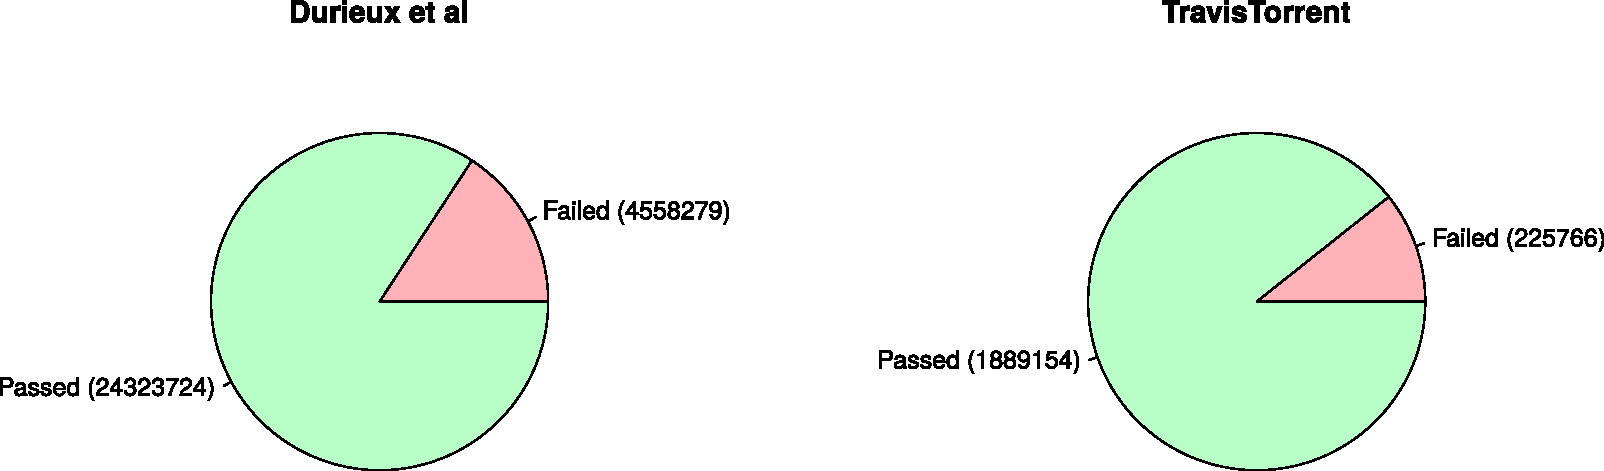
\includegraphics[width=\textwidth]{assets/charts/rq1-failure-probability.pdf}
	\caption{Probability of test run failure}
	\label{fig:rq1-failure-probability}
\end{figure}

\subsection{RQ2: Probability of consecutive failure}
In order to find consecutive failures, only the TravisTorrent project can be used as every entry in this dataset contains the identifier of the previous build which is required to link consecutive builds. The dataset contains $\SI{211040}{}$ test runs of which the test suite of the preceding test run was both executed and contained at least one failed test case. As illustrated in \autoref{fig:rq2-consecutive-failure}, $\SI{109224}{}$ of these test runs failed as well, versus $\SI{101816}{}$ test runs ($\SI{51.76}{\percent}$) that did succeed.

\begin{figure}[htbp!]
	\centering
	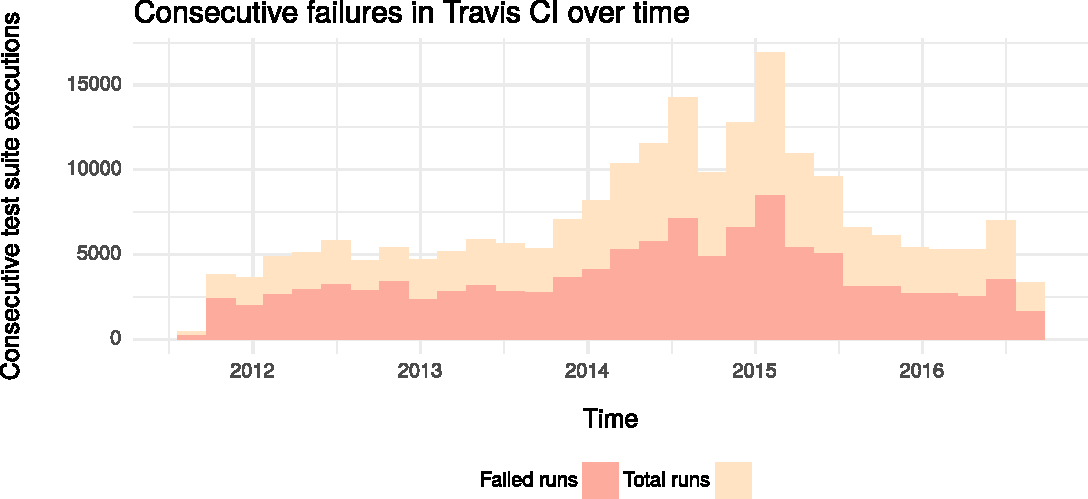
\includegraphics[width=\textwidth]{assets/charts/rq2-consecutive-failure.pdf}
	\caption{Consecutive test run failures on \travisci{}}
	\label{fig:rq2-consecutive-failure}
\end{figure}

\subsection{RQ3: Average test run duration}
The \travisci{} dataset provided by Durieux et al \cite{travisanalysis} has been filtered to exclude test runs with an execution time of less than $\SI{10}{\second}$, as this generally implies that the test suite did not actually execute due to an initialisation failure. \autoref{tbl:rq3-characteristics} contains the characteristics of the remaining analysed test runs. This table suggests that \travisci{} is primarily used for small projects, yet the maximal value is a strong outlier. \autoref{fig:rq3-durations} confirms the existence of $\SI{71378}{}$ test runs with an execution time of more than one hour. Further investigation has pointed out that these are mostly projects which are using mutation testing (\autoref{sssec:mutation-testing}), such as \texttt{plexus/yaks}\footnote{A Ruby library for hypermedia (\url{https://github.com/plexus/yaks}).}.

\begin{table}[h]
	\centering
	\begin{tabularx}{\textwidth}{|C|C|C|C|C|}
		\hline
		\textbf{\# runs} & \textbf{Minimum} & \textbf{Mean} & \textbf{Median} & \textbf{Maximum}\\
		\hline
		$\SI{24320504}{}$ & $\SI{10}{\second}$ & $\SI{385}{\second}$ & $\SI{178}{\second}$ & $\SI{26}{\hour} \SI{11}{\minute} \SI{26}{\second}$\\
		\hline
	\end{tabularx}
	\caption{Characteristics of the test run durations in \cite{travisanalysis}.}
	\label{tbl:rq3-characteristics}
\end{table}

\begin{figure}[htbp!]
	\centering
	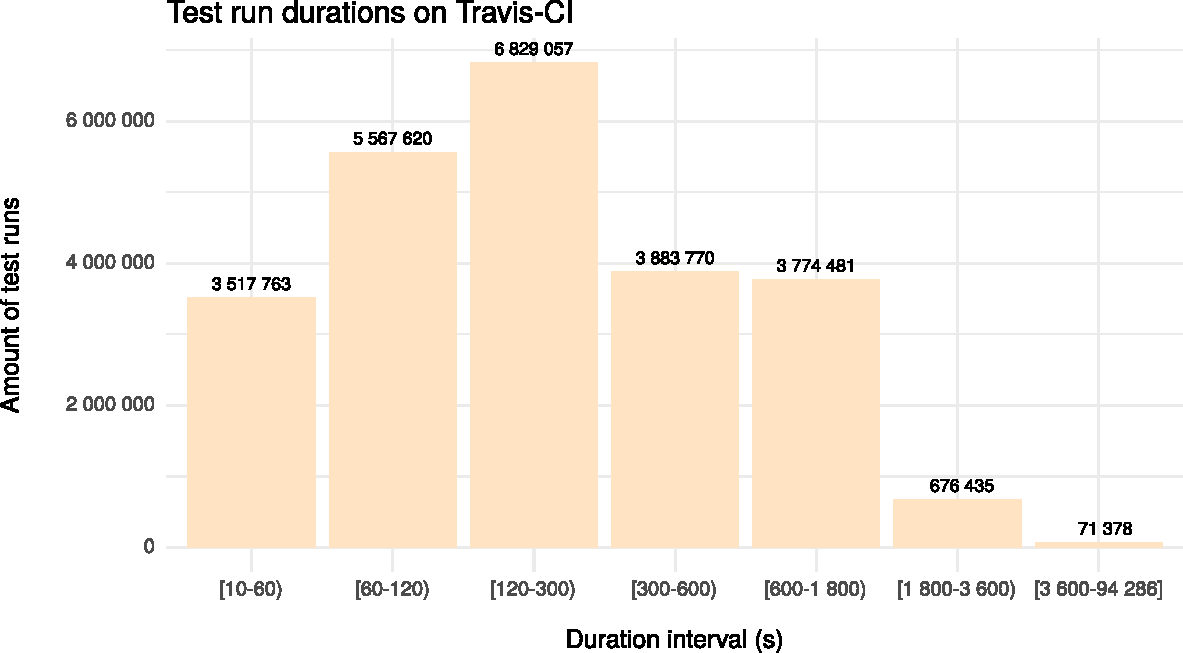
\includegraphics[width=\textwidth]{assets/charts/rq3-test-run-durations.pdf}
	\caption{Test run durations on \travisci{}}
	\label{fig:rq3-durations}
\end{figure}


\subsection{RQ4: Applying \tcp{} to Dodona}
Given the $\SI{62}{}$ collected test runs, another $\SI{9}{}$ runs have been omitted because these have been identified as a bug in the configuration of the test suite, preventing any test to be executed at all. This is something which cannot be detected by a prioritisation framework, since this requires more contextual information about the project.\\

\noindent \autoref{fig:rq4-performance} compares the performance of respectively the Alpha algorithm, the Greedy algorithm, the HGS algorithm and the ROCKET algorithm to the original, non-prioritised execution. The Alpha and HGS algorithm provide the most accurate predictions, with the latter algorithm being the least consistent. The Greedy algorithm on the other hand succeeds in predicting some executions very accurately, while failing to predict other runs anywhere near, which is the expected behaviour of a greedy heuristic. Finally, the ROCKET algorithm is not suitable for this project.\\

\begin{figure}[htbp!]
\centering
\subfloat[Alpha algorithm]{%
	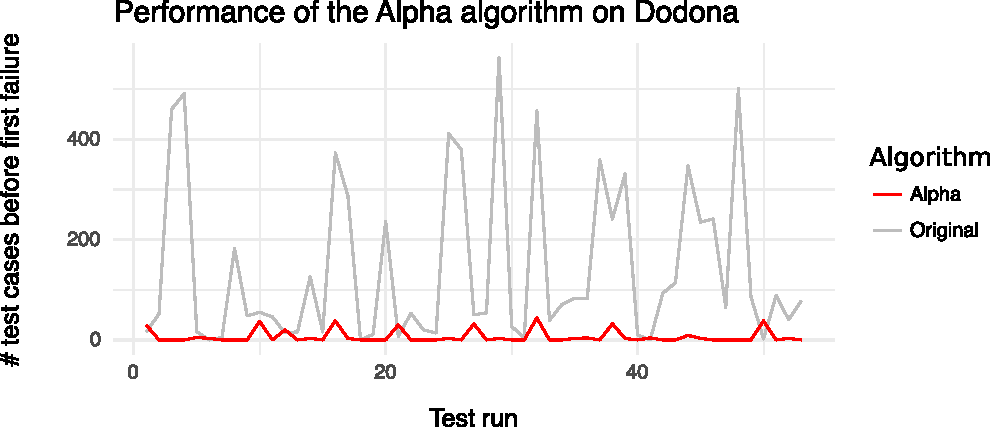
\includegraphics[width=\textwidth]{assets/charts/rq4-dodona-alpha.pdf}
}
\end{figure}
\begin{figure}
\ContinuedFloat
\subfloat[Greedy algorithm]{%
	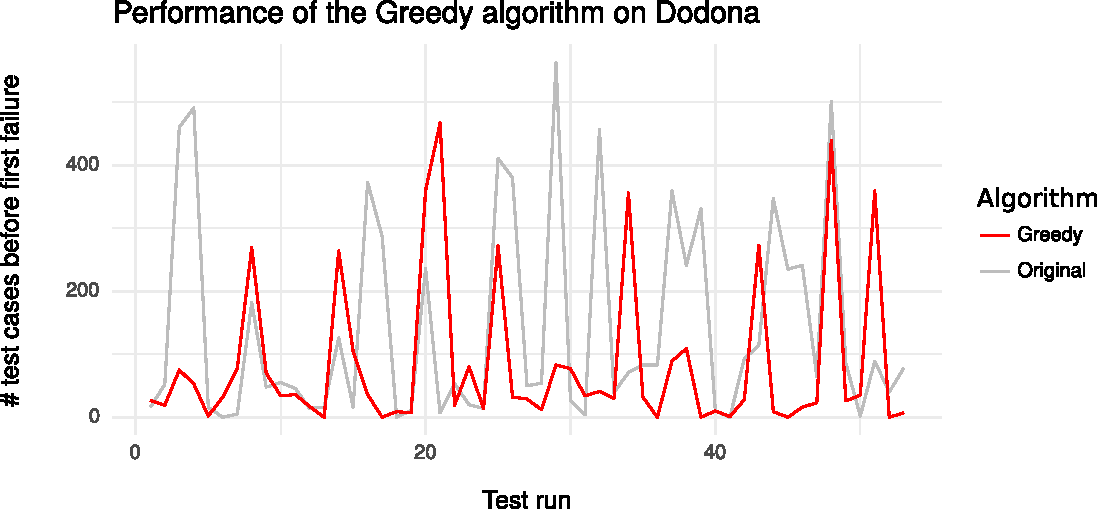
\includegraphics[width=\textwidth]{assets/charts/rq4-dodona-greedy.pdf}
}
\end{figure}
\begin{figure}
\ContinuedFloat
\subfloat[HGS algorithm]{%
	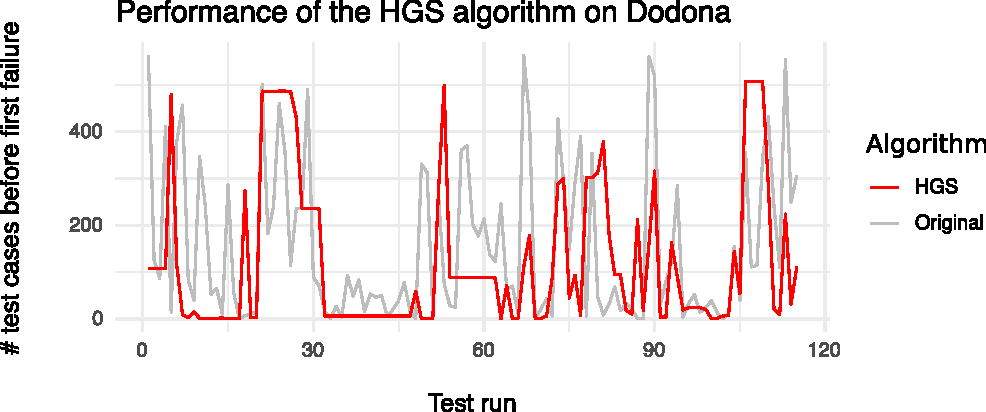
\includegraphics[width=\textwidth]{assets/charts/rq4-dodona-hgs.pdf}
}
\end{figure}
\begin{figure}
\ContinuedFloat
\centering
\subfloat[ROCKET algorithm]{%
	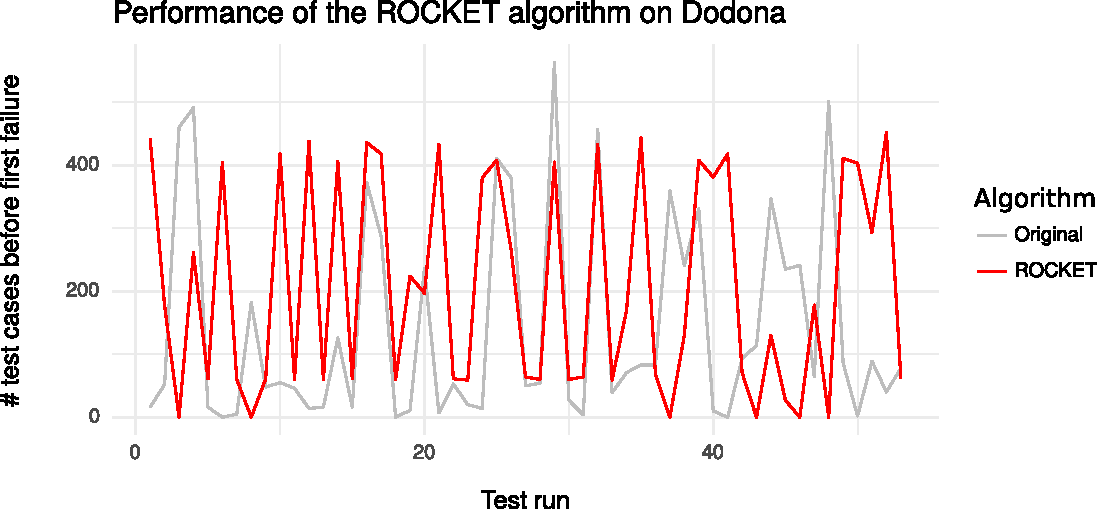
\includegraphics[width=\textwidth]{assets/charts/rq4-dodona-rocket.pdf}
}
\caption{Prediction performance on the Dodona project}
\label{fig:rq4-performance}
\end{figure}

\noindent \autoref{tbl:rq4-first-failure} contains the minimum, mean, median and maximum median amount of test cases until the first failure is observed. This table indicates that, except for the GreedyCoverAffected algorithm\footnote{The AllInOrder algorithm can be considered a deterministic random algorithm and therefore not an actual predictor.}, every predictor is able to perform at least one successful prediction. Furthermore, the maximum amount of executed test cases is lower than the original, for every predictor. The previous paragraph has already observed that the Alpha and HGS algorithm provide the best prediction accuracy for Dodona, this hypothesis is confirmed by the low median and mean values for these algorithms. These values confirm as well that the ROCKET algorithm is not able of providing accurate predictions.

\begin{table}[h]
	\centering
	\begin{tabularx}{\textwidth}{|X||c|c|c|c|}
		\hline
		\textbf{Algorithm} & \textbf{Minimum} & \textbf{Mean} & \textbf{Median} & \textbf{Maximum}\\
		
		\hline
		
		\emph{Original} & $\SI{0}{}$ & $\SI{143}{}$ & $\SI{65}{}$ & $\SI{563}{}$\\
		
		\hline
		
		Alpha & $\SI{0}{}$ & $\SI{7}{}$ & $\SI{6}{}$ & $\SI{44}{}$\\
		
		\hline
		AffectedRandom & $\SI{0}{}$ & $\SI{82}{}$ & $\SI{18}{}$ & $\SI{428}{}$\\
		AllInOrder & $\SI{1}{}$ & $\SI{102}{}$ & $\SI{71}{}$ & $\SI{455}{}$\\
		AllRandom & $\SI{0}{}$ & $\SI{71}{}$ & $\SI{16}{}$ & $\SI{477}{}$\\
		
		\hline
		
		GreedyCoverAffected & $\SI{31}{}$ & $\SI{307}{}$ & $\SI{296}{}$ & $\SI{446}{}$\\
		GreedyCoverAll & $\SI{0}{}$ & $\SI{85}{}$ & $\SI{32}{}$ & $\SI{467}{}$\\
		GreedyTimeAll & $\SI{0}{}$ & $\SI{209}{}$ & $\SI{172}{}$ & $\SI{452}{}$\\
		
		\hline
		
		HGSAffected & $\SI{0}{}$ & $\SI{54}{}$ & $\SI{10}{}$ & $\SI{511}{}$\\
		HGSAll & $\SI{0}{}$ & $\SI{109}{}$ & $\SI{6}{}$ & $\SI{487}{}$\\
		
		\hline
		
		ROCKET & $\SI{0}{}$ & $\SI{208}{}$ & $\SI{170}{}$ & $\SI{452}{}$\\
		
		\hline
	\end{tabularx}
	\caption{Amount of executed test cases until the first failure.}
	\label{tbl:rq4-first-failure}
\end{table}

\noindent Similarly, \autoref{tbl:rq4-first-failure-duration} contains the minimum, mean, maximum and median duration until the first failed test case is observed. This data further confirms the observations made in the previous paragraph and the effectiveness of the GreedyTimeAll predictor. Notice that the ROCKET algorithm performs better time-wise than quantity wise.

\begin{table}[h]
	\centering
	\begin{tabularx}{\textwidth}{|X||c|c|c|c|}
		\hline
		\textbf{Algorithm} & \textbf{Minimum} & \textbf{Mean} & \textbf{Median} & \textbf{Maximum}\\
		
		\hline
		
		\emph{Original} & $\SI{0}{\second}$ & $\SI{154}{\second}$ & $\SI{125}{\second}$ & $\SI{622}{\second}$\\
		
		\hline
		
		Alpha & $\SI{0}{\second}$ & $\SI{5}{\second}$ & $\SI{0}{\second}$ & $\SI{84}{\second}$\\
		
		\hline
		AffectedRandom & $\SI{0}{\second}$ & $\SI{64}{\second}$ & $\SI{10}{\second}$ & $\SI{355}{\second}$\\
		AllInOrder & $\SI{0}{\second}$ & $\SI{177}{\second}$ & $\SI{171}{\second}$ & $\SI{456}{\second}$\\
		AllRandom & $\SI{0}{\second}$ & $\SI{64}{\second}$ & $\SI{11}{\second}$ & $\SI{611}{\second}$\\
		
		\hline
		
		GreedyCoverAffected & $\SI{6}{\second}$ & $\SI{123}{\second}$ & $\SI{109}{\second}$ & $\SI{264}{\second}$\\
		GreedyCoverAll & $\SI{0}{\second}$ & $\SI{60}{\second}$ & $\SI{25}{\second}$ & $\SI{306}{\second}$\\
		GreedyTimeAll & $\SI{0}{\second}$ & $\SI{44}{\second}$ & $\SI{15}{\second}$ & $\SI{178}{\second}$\\
		
		\hline
		
		HGSAffected & $\SI{0}{\second}$ & $\SI{58}{\second}$ & $\SI{6}{\second}$ & $\SI{581}{\second}$\\
		HGSAll & $\SI{0}{\second}$ & $\SI{130}{\second}$ & $\SI{16}{\second}$ & $\SI{578}{\second}$\\
		
		\hline
		
		ROCKET & $\SI{0}{\second}$ & $\SI{47}{\second}$ & $\SI{16}{\second}$ & $\SI{178}{\second}$\\
		
		\hline
	\end{tabularx}
	\caption{Duration until the first failure.}
	\label{tbl:rq4-first-failure-duration}
\end{table}

    duration         Original        AllRandom     
Min.   :118165   Min.   :  0.00   Min.   : 0.000  
1st Qu.:195877   1st Qu.:  0.00   1st Qu.: 0.000  
Median :297371   Median :  2.00   Median : 4.000  
Mean   :303527   Mean   : 67.57   Mean   : 9.257  
3rd Qu.:414956   3rd Qu.:110.00   3rd Qu.:13.500  
Max.   :505996   Max.   :278.00   Max.   :64.000  

AllInOrder     GreedyCoverAll   AffectedRandom  
Min.   : 0.000   Min.   : 0.000   Min.   : 0.000  
1st Qu.: 0.000   1st Qu.: 0.000   1st Qu.: 0.000  
Median : 1.000   Median : 1.000   Median : 2.000  
Mean   : 9.229   Mean   : 8.971   Mean   : 8.886  
3rd Qu.:12.000   3rd Qu.:13.000   3rd Qu.:11.500  
Max.   :37.000   Max.   :44.000   Max.   :45.000  

HGSAffected     GreedyCoverAffected     HGSAll    
Min.   : 0.000   Min.   : 0.00       Min.   : 0.0  
1st Qu.: 0.000   1st Qu.: 0.00       1st Qu.: 0.0  
Median : 3.000   Median : 2.00       Median : 7.0  
Mean   : 8.886   Mean   :15.09       Mean   : 9.6  
3rd Qu.:11.500   3rd Qu.:31.00       3rd Qu.:12.5  
Max.   :64.000   Max.   :43.00       Max.   :43.0  

Alpha            Rocket       GreedyTimeAll   
Min.   : 0.000   Min.   :  0.00   Min.   :  0.00  
1st Qu.: 0.000   1st Qu.:  3.50   1st Qu.:  3.50  
Median : 1.000   Median : 27.00   Median : 27.00  
Mean   : 8.971   Mean   : 42.23   Mean   : 42.23  
3rd Qu.:13.000   3rd Qu.: 49.00   3rd Qu.: 49.00  
Max.   :44.000   Max.   :216.00   Max.   :216.00  

Original\_ms      AllRandom\_ms    AllInOrder\_ms   
Min.   :     0   Min.   :     0   Min.   :     0  
1st Qu.:     0   1st Qu.:     0   1st Qu.:     0  
Median :  9560   Median :   739   Median :   862  
Mean   : 73612   Mean   : 13299   Mean   : 32391  
3rd Qu.:122586   3rd Qu.: 13592   3rd Qu.: 78063  
Max.   :283433   Max.   :184805   Max.   :139345  

GreedyCoverAll\_ms AffectedRandom\_ms HGSAffected\_ms  
Min.   :     0    Min.   :     0    Min.   :     0  
1st Qu.:     0    1st Qu.:     0    1st Qu.:     0  
Median :   620    Median :   317    Median :  1318  
Mean   : 15251    Mean   : 19732    Mean   : 23738  
3rd Qu.:  8620    3rd Qu.:  6460    3rd Qu.: 11786  
Max.   :197463    Max.   :174491    Max.   :211702  

GreedyCoverAffected\_ms   HGSAll\_ms         Alpha\_ms     
Min.   :    0          Min.   :     0   Min.   :     0  
1st Qu.:    0          1st Qu.:     0   1st Qu.:     0  
Median : 4229          Median :  2818   Median :   647  
Mean   :21835          Mean   : 12494   Mean   : 15189  
3rd Qu.:37885          3rd Qu.:  8475   3rd Qu.:  8386  
Max.   :75637          Max.   :157003   Max.   :193618  

Rocket\_ms      GreedyTimeAll\_ms      idx      
Min.   :     0   Min.   :    0    Min.   : 1.0  
1st Qu.:     0   1st Qu.:    0    1st Qu.: 9.5  
Median :   254   Median :  257    Median :18.0  
Mean   :  6844   Mean   : 6852    Mean   :18.0  
3rd Qu.:  1760   3rd Qu.: 1754    3rd Qu.:26.5  
Max.   :100011   Max.   :99765    Max.   :35.0  

	% !TeX root = thesis.tex

\chapter{Conclusion}

The main purpose of this thesis has been to investigate different approaches towards optimising the test suite of a common software project. The concepts of \tsm{}, \tcs{} and \tcp{} have been introduced and accompanying algorithms have been presented. A novel client-server oriented framework for the latter approach has been proposed, as well as a new prioritisation algorithm. Finally, \velocity{} has been applied to the UGent Dodona project, proving its ability to predict test case failure and therefore reduce the execution time of the test suite.\\

\noindent A second purpose of this thesis was to gain useful insights into the behaviour of a typical test suite. These insights have been formulated as three additional research questions, to which answers have been provided in the previous chapter.

\section{Future work}
The proposed \velocity{} implementation in this thesis is currently able to prioritise a Gradle Java project using 10 available predictors and a meta predictor. While this is certainly functional, it is far from complete and multiple improvements can be added.

\subsection{Java Agent}
The existing Java Agent can be extended in multiple ways. The most prominent addition would be to allow test cases to be executed in parallel. At the moment of writing, this is not possible yet. In order to facilitate parallel testing, one must first decide how to schedule the prioritised test cases across multiple threads, since the execution time of a test case varies strongly. One possibility to perform this scheduling is to use the average execution time per test case, which is obtained from prior runs. Alternatively, this can be performed at runtime by using any existing inter-thread communication paradigm such as message passing. On the implementation side of parallelisation, the current \texttt{TestProcessor} should be adapted to inherit from the \texttt{MaxNParallelTestClassProcessor}. A thread pool should ideally be used to reduce the overhead of restarting a new thread for every test case.

\subsection{Predictions}
Further research and improvements to the predictors can be made on four different aspects.\\

\noindent The first enhancement is that currently the predictor does not discriminate between a unit test or an integration test. 
Recall that the scope of a unit test is limited to a small fraction of the application and that its execution time is ideally rather low. An integration test however usually takes longer to execute and tests multiple components of the application at once. The predictor could make use of this distinction and assume that a failure in a unit test has a high probability of resulting in a failed integration test as well, hence prioritising unit tests over integration tests.\\

\noindent Secondly, the prediction algorithms currently take into account which source code lines have either been modified or removed in order to prioritise affected test cases. Likewise, test cases of which the code has been modified should also be considered as candidates for prioritisation, as the changed test case might contain a bug as well.\\

\noindent A third and unexplored research opportunity is to investigate the joint performance of multiple prediction algorithms combined. This could be integrated with the existing meta predictor. Instead of assigning a score to the entire prediction, multiple predictions could be intermingled using predefined weights.\\

\noindent The final improvement is to take into account branch coverage in addition to the statement coverage which is currently used. This is a rather complex feature as not every coverage framework is capable of reporting accurately which branches have been covered and which ones have not. A suggested implementation would be to instrument the source code and rewrite every condition of every branch as separate \texttt{if}-statements.

\subsection{Meta predictor}
The proposed meta predictor increases the score of every predictor which predicted an above-average ranking and decreases the score of the other predictors. However, a possible problem with this approach is that the nature of the source code might evolve and change as time progresses. Using the current updating strategy it will take several test suite invocations for an alternative predictor to be preferred by the meta predictor. If a saturating counter would be used instead (\autoref{fig:saturating-counter}), this would be resolved much more quickly, allowing a more versatile meta predictor.

\begin{figure}[htbp!]
	\centering
	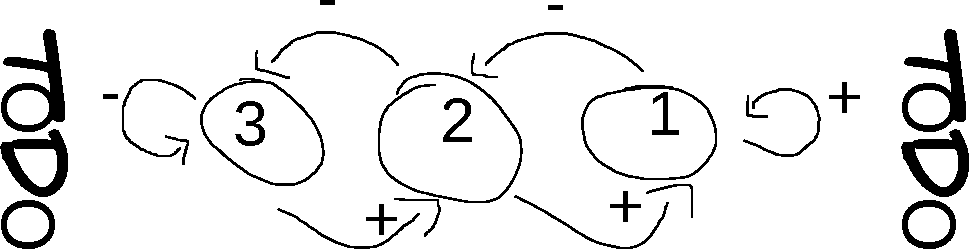
\includegraphics[width=\textwidth]{assets/images/saturating-counter.pdf}
	\caption{Saturating counter}
	\label{fig:saturating-counter}
\end{figure}

In addition to implementing a different update strategy, it might be worth to investigate the use of machine learning or linear programming models as a meta predictor, or even as a prediction algorithm.

\subsection{Final enhancements}
Finally, since some of the implemented algorithms are inherently \tsm{} algorithms rather than prioritisation algorithms, the framework might opt to not execute some test cases at all, whereas now the entire test suite is always executed.\\

\noindent Support for other programming languages and frameworks is possible by implementing new agents. The basic implementation is straightforward to restart the test suite after every executed test case, should test case reordering not be supported natively by the test framework.
	
	\bibliographystyle{phdsymp}
	\bibliography{references}
\end{document}